\chapter{Проектируем параллельное (concurrent) приложение}
\label{designing-a-concurrent-application}
\begin{wrapfigure}{r}{0.35\linewidth}
    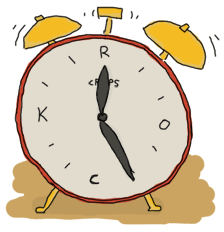
\includegraphics[width=1\linewidth]{clock.png}
\end{wrapfigure}
Всё это, конечно, здорово.
Вы ознакомились с базовыми принципами, но, опять же, мы с самого начала книги занимались лишь игрушечными примерами: калькуляторами, деревьями, ездили из Хитроу в Лондон и т.д.
Пора сделать что\--нибудь более интересное с точки зрения обучения.
Мы напишем небольшое приложение на параллельном (сoncurrent) Erlang.
Приложение будет простым и взаимодействие с ним будет осуществляться посредством строковых команд.
Кроме того, оно будет приносить пользу и его функциональность можно будет наращивать.

Меня нельзя назвать организованным человеком.
Я теряюсь в домашних заданиях, благоустройстве квартиры, этой книге, работе, совещаниях, встречах и прочем.
У меня есть дюжина списков с задачами, которые я забываю сделать, или просто не нахожу для них времени.
Надеюсь, вам тоже иногда нужно напоминать о делах (хоть ваш разум  и не блуждает так же часто как мой).
Мы напишем приложение, которое уведомляет вас о необходимости что\--либо сделать и напоминает о встречах.
\section{Разбираем задачу}
\label{understanding-the-problem}
Перво\--наперво нужно понять, что мы вообще собираемся сделать.
Вы скажете: <<Напоминалку>>.
<<Ну, конечно>>, \--- скажу я.
Но это только начало.
Как мы собираемся взаимодействовать с программой?
Что она должна для нас делать?
Как представить программу при помощи процессов?
Как узнать, какие нужно отсылать сообщения?

Как говорится: <<Ходить по воде и разрабатывать программное обеспечение по техническому заданию одинаково просто, если и то и другое заморожено.>>
Так что давайте разработаем технические условия и будем их придерживаться.
Наша программа позволит совершать следующие действия:
\begin{itemize}
\item Добавлять событие.
У событий может быть крайний срок исполнения (момент времени, о котором необходимо предупредить), наименование события и его описание.
\item Показывать предупреждение, когда подошло время.
\item Отменять событие по его имени.
\item Не хранить данные на диске.
    Для демонстрации архитектурных концепций, которые мы рассмотрим, хранение совершенно излишне.
Для настоящего приложения это, конечно никуда не годится, но я покажу, куда можно вставить код, если вам захочется реализовать эту функциональность, и укажу на несколько полезных функций, которые могли бы вам в этом помочь.
\item Так как постоянного хранилища у нас нет, нам нужно иметь возможность изменять код во время исполнения.
\item Общение с программой будет осуществляться через командную строку, но мы должны предусмотреть возможность последующего расширения  средств взаимодействия (добавить, скажем, графический интерфейс, доступ через веб\--страницу, через систему обмена мгновенными сообщениями (instant messaging), электронную почту и прочее).
\end{itemize}

Для нашей программы я избрал такой способ организации:
\begin{figure}[h!]
    \centering
    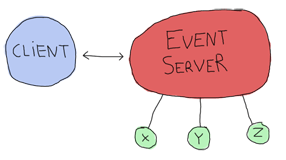
\includegraphics[width=0.4\textwidth]{reminder-structure.png}
\end{figure}

Где клиент, сервер событий и x, y, z представлены в виде процессов.
Вот что каждый из них может делать:
\subsection{Сервер событий}
\label{event-server}
\begin{itemize}
\item Принимает подписки от клиентов.
\item Передаёт уведомления от процессов, генерирующих события, каждому подписчику.
\item Принимает сообщения о добавлении событий (и необходимости запуска процессов x, y, z).
\item Может принимать сообщения об отмене события, и последующем убийстве процессов\--генераторов событий.
\item Может быть остановлен клиентом.
\item Его код может быть перезагружен из оболочки.
\end{itemize}
\subsection{Клиент}
\label{client}
\begin{itemize}
\item Подписывается на события у сервера событий и получает уведомления посредством сообщений.
Используя этот механизм, можно легко спроектировать группу клиентов, которые создают подписку на сервере событий.
Каждый клиент потенциально может служить шлюзом к различным точкам взаимодействия, упомянутым выше (графический интерфейс, веб\--страница, программа обмена мгновенными сообщениями, электронная почта и т.д.).
\item Запрашивает у сервера создание события с необходимыми параметрами.
\item Совершает к серверу запрос на отмену события.
\item Отслеживает сервер (на случай если тот прекратит работу).
\item При необходимости останавливает сервер событий.
\end{itemize}
\subsection{x, y и z}
\label{x-y-and-z}
\begin{itemize}
\item С их помощью обозначаются уведомления, готовые к запуску (они реализованы в виде таймеров, связанных с сервером событий).
\item Отсылают сообщение серверу событий по истечении заданного периода.
\item Получают сообщение об отмене и умирают.
\end{itemize}

Обратите внимание, что все клиенты (IM, почта и т.д., которые в этой книге не реализованы) получают уведомления обо всех событиях, а отмена не входит в список вещей, о которых следует предупреждать клиентов.
Эта программа написана для нас с вами, поэтому предполагается, что её будет запускать только один пользователь.

Вот более сложная схема, с указанием всех возможных сообщений:
\begin{figure}[h!]
    \centering
    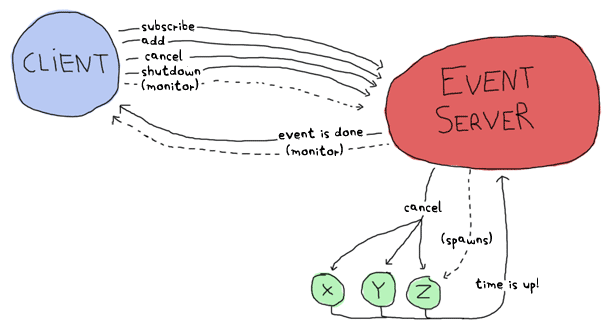
\includegraphics[width=0.7\textwidth]{reminder-bubbles-and-arrows.png}
\end{figure}

Здесь указан каждый процесс, который мы будем использовать.
Стрелки обозначают передаваемые сообщения.
С их помощью мы записали высокоуровневый протокол взаимодействия, ну или хотя бы его основу.

Нужно заметить, что для уведомлений мы используем по процессу на каждое событие.
Это слишком расточительно, и такое решение будет плохо масштабироваться в реальной задаче.
Но для приложения, единственным пользователем которого будете только вы, это вполне уместно.
Можно было бы решить эту проблему иначе, и использовать, к примеру, функцию \href{http://erldocs.com/R15B/stdlib/timer.html\#send_after/2}{timer:send\_after/2-3}, позволив тем самым избежать порождения большого количества процессов.
\clearpage
\section{Определяем протокол}
\label{defining-the-protocol}
Теперь, когда мы знаем что должен передавать каждый компонент и каковы его функции, неплохо было бы составить список всех передаваемых сообщений, и установить их вид.
Начнём с взаимодействия между клиентом и сервером событий:
\begin{figure}[h!]
    \centering
    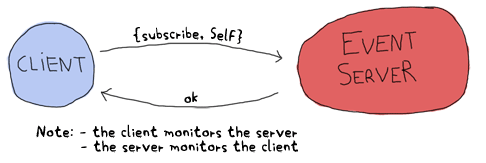
\includegraphics[width=0.6\textwidth]{reminder-subscribe.png}
\end{figure}

Я решил использовать два монитора, так как между клиентом и сервером нет явной зависимости.
Конечно, клиент без сервера работать не сможет, но сервер без клиента будет существовать без проблем.
Здесь можно было бы использовать связь (link), но мы хотим, чтобы функциональность нашей системы могла расширяться за счёт различных клиентов, поэтому мы не можем просто предположить, что после остановки сервера любой клиент тоже захочет аварийно завершиться.
Мы также не можем рассчитывать на то, что клиента можно превратить в системный процесс, и он начнёт улавливать завершения (exits) в случае смерти сервера.
Перейдём к следующему набору сообщений:
\begin{figure}[h!]
    \centering
    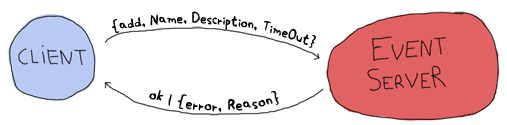
\includegraphics[width=0.6\textwidth]{reminder-add.png}
\end{figure}

Здесь мы добавляем на сервере событий ещё одно событие.
Клиенту высылается подтверждение в виде атома \ops{ok}, за исключением случаев, когда что\--то пошло не так (например, TimeOut был передан в неверном формате.)
Обратная операция удаления событий может быть совершена следующим образом:
\begin{figure}[h!]
    \centering
    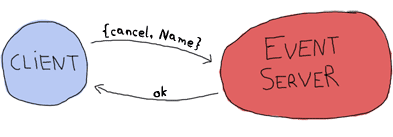
\includegraphics[width=0.6\textwidth]{reminder-remove.png}
\end{figure}

Позже сервер событий может отослать уведомление о том, что событие наступило:
\begin{figure}[h!]
    \centering
    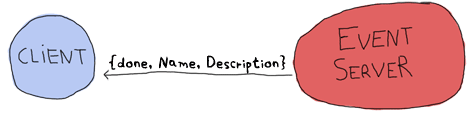
\includegraphics[width=0.6\textwidth]{reminder-cs-done.png}
\end{figure}

Нам осталось определить пару особых случаев: когда необходимо остановить сервер, и когда сервер аварийно завершается:
\begin{figure}[h!]
    \centering
    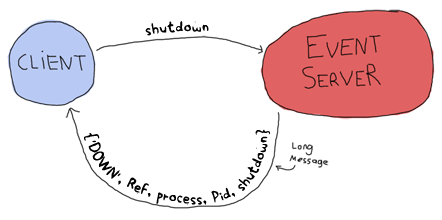
\includegraphics[width=0.6\textwidth]{reminder-shutdown.png}
\end{figure}

Прямое подтверждение об остановке  сервера не отсылается, так как о случившемся нас предупредит монитор.
Вот, в общем\--то и всё, что будет происходить между клиентом и сервером событий.
Перейдём к сообщениям, передаваемым между сервером событий и самими процессами событий.

Перед тем как мы приступим к их описанию, я бы хотел заметить, что неплохо было бы установить связи (links)  между сервером событий и событиями.
Сделать это нужно по той причине, что если сервер умирает, нам нужно чтобы все события умерли вместе с ним \--- без сервера в их существовании нет никакого смысла.

Итак, вернёмся к событиям.
Когда сервер событий их создаёт, он присваивает каждому особый идентификатор (имя события).
Как только приходит время какого\--нибудь события, сервер должен отослать об этом уведомление:
\begin{figure}[h!]
    \centering
    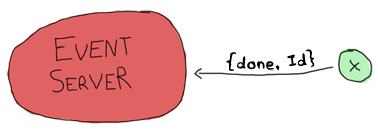
\includegraphics[width=0.6\textwidth]{reminder-es-done.png}
\end{figure}

\clearpage
Событие, в свою очередь, должно ожидать от сервера событий сигналы об отмене:
\begin{figure}[h!]
    \centering
    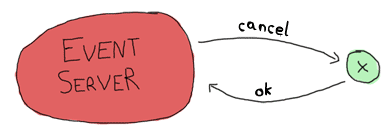
\includegraphics[width=0.6\textwidth]{reminder-cancel.png}
\end{figure}

Вот и всё.
Последний штрих - нам потребуется сообщение, которое позволит обновлять код сервера:
\begin{figure}[h!]
    \centering
    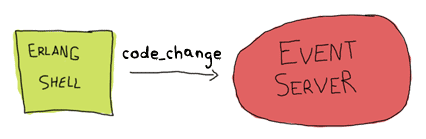
\includegraphics[width=0.6\textwidth]{reminder-code-change.png}
\end{figure}

Отвечать на это сообщение нет необходимости.
Когда мы реализуем эту часть нашей программы, вы поймёте, почему мы можем так сделать.

Теперь у нас есть и протокол общения, и приблизительная структура иерархии процессов.
Можно наконец\--то приступить к воплощению нашего проекта в жизнь.
\section{Заложим\--ка основы}
\label{lay-them-foundations}
\begin{wrapfigure}{r}{0.4\linewidth}
    
\includegraphics[width=1\linewidth]{cement.png}
\end{wrapfigure}
Для начала мы должны создать стандартный набор директорий, принятый в Erlang.
Вот как он выглядит:

ebin/

include/

priv/

src/

В директорию \ops{ebin/} попадают скомпилированные файлы.
Директория \ops{include/} используется для хранения файлов \ops{.hrl}, предназначенных для включения другими приложениями; файлы с расширением \ops{.hrl}, доступные лишь текущему приложению (private), обычно хранятся в директории \ops{src/}.
Директория \ops{priv/} содержит исполняемые файлы, которые могут взаимодействовать с Erlang.
К их числу относятся некоторые драйверы и прочее в этом духе.
В нашем проекте мы эту директорию использовать не будем.
Ну и последняя директория \--- \ops{src/}, в ней находятся все файлы \ops{.erl}.

Описанная структура директорий может немного варьироваться в стандартных проектах Erlang.
Для хранения некоторых конфигурационных файлов может добавляться директория \ops{conf/}, для документации \ops{doc/} и \ops{lib/} \--- для сторонних библиотек, которые ваше приложение использует во время исполнения.
Зачастую различные Erlang\--продукты, представленные на рынке, используют имена отличные от указанных, но четыре имени, упомянутые выше, обычно не меняются, так как они являются частью \href{http://www.erlang.org/doc/design_principles/applications.html\#id71171}{стандартных приёмов (standard practices) OTP}.
\section{Модуль для работы с событиями}
\label{an-event-module}
Зайдите в директорию \ops{src/} и откройте модуль \href{http://learnyousomeerlang.com/static/erlang/event.erl}{event.erl}, который реализует события x, y и z, отмеченные на приведённых ранее рисунках.
Я начинаю именно с этого модуля, так как у него меньше всего зависимостей.
Мы сможем попытаться его запустить, не реализовывая сервер событий или функции клиента.

Перед тем как мы начнём писать код, я должен упомянуть, что разработанный нами протокол неполон.
Он помогает представить те данные, которые будут пересылаться между процессами, но не описывает подробности пересылки.
Как работает адресация? 
Что мы при этом используем \--- ссылки или имена и т.д.
Большинство сообщений будут завёрнуты в кортеж вида \ops{\{Pid, Ref, Message\}}, где \emph{Pid} \--- отправитель и \emph{Ref} \--- уникальный идентификатор сообщения, который помогает определить, от кого был получен ответ.
Если бы перед ожиданием ответов мы отослали множество сообщений, то без ссылок нам не удалось бы понять, какому сообщению соответствует каждый из ответов.

Начинаем.
Ядром процессов, исполняющих код модуля \ops{event.erl} будет функция \ops{loop/1}, основа которой будет выглядеть приблизительно следующим образом, если вы помните протокол:
\begin{lstlisting}[style=erlang]
loop(State) ->
    receive
        {Server, Ref, cancel} ->
            ...
    after Delay ->
        ...
    end.
\end{lstlisting}

Здесь показан поддерживаемый нами тайм\--аут, который оповещает о наступлении события, а также способ отмены события сервером.
В цикле вы можете заметить переменную \emph{State}.
Эта переменная будет содержать значение тайм\--аута (в секундах) и имя события (необходимое для отсылки сообщения \ops{\{done, Id\}}.)
Чтобы отсылать уведомления серверу событий, нам также понадобится его pid.

Вся эта информация вполне годится для размещения в состоянии цикла.
Для этого объявим в начале файла запись \ops{state}:
\begin{lstlisting}[style=erlang]
-module(event).
-compile(export_all).
-record(state, {server,
                name="",
                to_go=0}).
\end{lstlisting}

Состояние объявлено, теперь можно немного усовершенствовать цикл:
\begin{lstlisting}[style=erlang]
loop(S = #state{server=Server}) ->
    receive
        {Server, Ref, cancel} ->
            Server ! {Ref, ok}
    after S#state.to_go*1000 ->
        Server ! {done, S#state.name}
    end.
\end{lstlisting}

Умножение на тысячу используется для перевода значения \ops{to\_go} из секунд в миллисекунды.\\
\colorbox{lorange}
{
\begin{minipage}{1.0\linewidth}
    \textbf{Не забывайтесь:}\\
    Далее речь пойдёт о языковом недостатке!
    Переменная <<Server>> используется при сопоставлении с образцом в секции receive, и поэтому в заголовке функции я связываю её со значением.
    Помните, что \ref{records} ~записи \--- это хак!
    \ops{S\#state.server} тихонько разворачивается в выражение \ops{element(2, S)}, использовать которое в качестве шаблона для сопоставления не получится.

    Для выражения \ops{S\#state.to\_go}, следующего за \ops{after}, этот механизм срабатывает нормально, так как его вычисление можно отложить на потом.
\end{minipage}
}

А теперь проверим цикл:
\begin{lstlisting}[style=erlang]
6> c(event).
{ok,event}
7> rr(event, state).
[state]
8> spawn(event, loop, [#state{server=self(), name="test", to_go=5}]).
<0.60.0>
9> flush().
ok
10> flush().
Shell got {done,"test"}
ok
11> Pid = spawn(event, loop, [#state{server=self(), name="test", to_go=500}]).
<0.64.0>
12> ReplyRef = make_ref().
#Ref<0.0.0.210>
13> Pid ! {self(), ReplyRef, cancel}.
{<0.50.0>,#Ref<0.0.0.210>,cancel}
14> flush().
Shell got {#Ref<0.0.0.210>,ok}
ok
\end{lstlisting}

Довольно насыщенный пример.
Сначала мы импортируем запись (record) из модуля обработки событий командой \ops{rr(Mod)}.
Затем запускаем цикл обработки событий, для которого сервером выступает оболочка (\ops{self()}).
Заданное событие должно произойти через 5 секунд.
Выражение в 9\--ой строке было запущено через 3 секунды, в 10\--ой \--- через 6 секунд.
Как видите, со второй попытки мы получили сообщение \ops{\{done, "test"\}}.

Далее я пытаюсь воспользоваться командой отмены (для ввода которой c запасом выделяется 500 секунд).
Видно, как я создаю ссылку, посылаю сообщение и получаю ответ, используя ту же самую ссылку.
Так мы можем определить, что полученное сообщение \ops{ok} пришло именно от заявленного процесса, а не какого\--либо другого существующего в системе.

Сообщение отмены завёрнуто в ссылку, а сообщение \ops{done} \--- нет.
Делаем мы так просто потому, что не ожидаем получить \ops{done} от какого\--либо определённого процесса (сгодится любой, мы не будем проводить сопоставление в receive), и отвечать на это сообщение мы тоже не намерены.
Я бы хотел провести заранее ещё одну проверку.
Что произойдёт, если событие случится в следующем году?
\begin{lstlisting}[style=erlang]
15> spawn(event, loop, [#state{server=self(), name="test", to_go=365*24*60*60}]).
<0.69.0>
16>
=ERROR REPORT==== DD-MM-YYYY::HH:mm:SS ===
Error in process <0.69.0> with exit value: {timeout_value,[{event,loop,1}]}
\end{lstlisting}

Ой.
Кажется мы наткнулись на ограничение, обусловленное реализацей.
Оказывается на значение тайм\--аута в Erlang накладывается ограничение в 50 дней (в миллисекундах).
Может быть, эта особенность и не столь важна, но у меня есть целых три причины для демонстрации этой ошибки:
\begin{enumerate}
    \item Я напоролся на этот нюанс, когда глава была наполовину написана, и я разрабатывал и тестировал для неё сопровождающий модуль.
    \item Само собой разумеется, что Erlang не всегда идеально подходит для решения любой задачи.
       Здесь перед нами предстаёт результат использования таймеров способом, не предусмотренным разработчиками.
    \item Но это, в общем\--то, не проблема; давайте придумаем как обойти это ограничение.
\end{enumerate}

Я решил устранить этот недостаток при помощи функции, которая разделяла бы значение длинного тайм\--аута на несколько частей.
Функцию \ops{loop/1} тоже потребуется немного изменить.
Проще говоря, мы разделим временной промежуток на равные части по 49 дней (так как ограничение равно приблизительно 50 дням), а затем к этим равным частям добавим остаток.
Полная сумма значений в этом списке должна быть равна исходному временному отрезку:
\begin{lstlisting}[style=erlang]
%% Because Erlang is limited to about 49 days (49*24*60*60*1000) in
%% milliseconds, the following function is used
normalize(N) ->
    Limit = 49*24*60*60,
    [N rem Limit | lists:duplicate(N div Limit, Limit)].
\end{lstlisting}

Функция \ops{\href{http://erldocs.com/R15B/stdlib/lists.html\#duplicate/2}{lists:duplicate/2}} принимает вторым аргументом данное выражение и повторяет его столько раз, сколько задано значением первого аргумента (\ops{[a,a,a] = lists:duplicate(3, a)}).
Если бы мы передали функции \ops{normalize/1} значение \ops{98*24*60*60+4}, то она бы возвратила \ops{[4,4233600,423360]}.
Для поддержки нового формата, функция \ops{loop/2} принимает следующий вид:
\begin{lstlisting}[style=erlang]
%% Loop uses a list for times in order to go around the ~49 days limit
%% on timeouts.
loop(S = #state{server=Server, to_go=[T|Next]}) ->
    receive
        {Server, Ref, cancel} ->
            Server ! {Ref, ok}
    after T*1000 ->
        if Next =:= [] ->
            Server ! {done, S#state.name};
            Next =/= [] ->
            loop(S#state{to_go=Next})
        end
    end.
\end{lstlisting}

Можете попробовать её запустить, она будет работать как и прежде, но ко всему прочему сможет обрабатывать тайм\--ауты длиной в несколько лет.
Работает этот механизм следующим образом: функция извлекает из списка \ops{to\_go} первый элемент и переходит в состояние ожидания на период, равный значению этого элемента.
Когда ожидание окончено, проверяется, есть ли в списке следующий элемент.
Если список пуст, то тайм\--аут окончен, и сервер получает об этом уведомление.
В противном случае процесс повторяется для всех остальных элементов списка, до полного их исчерпания.

Было бы очень досадно, если каждый раз при запуске процесса\--события приходилось бы вручную вызывать что\--нибудь вроде \ops{event:normalize(N)}, особенно если учесть, что этот  обходной манёвр совсем не должен заботить программистов, использующих наш код.
Стандартное решение для этой проблемы \--- завести функцию \ops{init}, которая будет содержать инициализацию данных, необходимых для правильной работы функции цикла.
Раз уж мы об этом заговорили, давайте заодно добавим стандартные функции \ops{start} и \ops{start\_link}:
\begin{lstlisting}[style=erlang]
start(EventName, Delay) ->
    spawn(?MODULE, init, [self(), EventName, Delay]).
 
start_link(EventName, Delay) ->
    spawn_link(?MODULE, init, [self(), EventName, Delay]).
 
%%% Event's innards
init(Server, EventName, Delay) ->
    loop(#state{server=Server,
                name=EventName,
                to_go=normalize(Delay)}).
\end{lstlisting}

Теперь интерфейс стал намного чище.
Но прежде чем приступить к его тестированию, было бы неплохо иметь для единственного сообщения, которое мы можем посылать и отменять, свою собственную интерфейсную функцию: 
\begin{lstlisting}[style=erlang]
cancel(Pid) ->
    %% Monitor in case the process is already dead
    Ref = erlang:monitor(process, Pid),
    Pid ! {self(), Ref, cancel},
    receive
        {Ref, ok} ->
            erlang:demonitor(Ref, [flush]),
            ok;
        {'DOWN', Ref, process, Pid, _Reason} ->
            ok
    end.
\end{lstlisting}

А вот и новый трюк!
Я использую монитор для проверки существования процесса.
Если процесс уже умер, я не трачу время на бессмысленное ожидание, а сразу возвращаю \ops{ok}, как и указано в протоколе.
Если процесс отвечает ссылкой, я знаю, что он скоро умрёт: я убираю ссылку, так как необходимости в ней больше нет.
Обратите внимание, что я также указываю опцию \ops{flush}, которая удалит сообщение \ops{DOWN}, если оно было послано до момента отключения мониторинга.

Протестируем описанные функции:
\begin{lstlisting}[style=erlang]
17> c(event).
{ok,event}
18> f().
ok
19> event:start("Event", 0).
<0.103.0>
20> flush().
Shell got {done,"Event"}
ok
21> Pid = event:start("Event", 500).
<0.106.0>
22> event:cancel(Pid).
ok
\end{lstlisting}

И они работают!
Осталась последняя особенность модуля событий, которая нас беспокоит \--- нам необходимо указывать оставшееся время в секундах.
Было бы намного удобнее использовать время в стандартном формате, таком как datetime в Erlang (\ops{\{\{Year, Month, Day\}, \{Hour, Minute, Second\}\}}).
Просто добавим следующую функцию, которая будет вычислять разницу между текущим временем на вашем компьютере и введённой задержкой:
\begin{lstlisting}[style=erlang]
time_to_go(TimeOut={{_,_,_}, {_,_,_}}) ->
    Now = calendar:local_time(),
    ToGo = calendar:datetime_to_gregorian_seconds(TimeOut) -
        calendar:datetime_to_gregorian_seconds(Now),
    Secs = if ToGo > 0  -> ToGo;
            ToGo =< 0 -> 0
        end,
    normalize(Secs).
\end{lstlisting}

Да уж, у функций в \href{http://erldocs.com/R15B/stdlib/calendar.html}{календарном модуле} прикольные имена.
Как было отмечено выше, этот код вычисляет число секунд между текущим моментом и моментом, когда должно произойти событие.
Если событие уже прошло, мы возвращаем 0, чтобы как можно быстрее уведомить об этом сервер.
Исправьте функцию init, чтобы она вызывала этот код вместо \ops{normalize/1}.
Также можно переименовать переменную \emph{Delay} в, скажем, \emph{DateTime}, если хотите, чтобы имя лучше описывало смысл происходящего:
\begin{lstlisting}[style=erlang]
init(Server, EventName, DateTime) ->
    loop(#state{server=Server,
        name=EventName,
        to_go=time_to_go(DateTime)}).
\end{lstlisting}

Всё, с этим закончили.
Теперь можно сделать перерыв, создать новое событие, сходить выпить пинту (пол\--литра) молока/пива и вернуться точно к моменту, когда придёт сообщение о том, что событие наступило.
\section{Сервер событий}
\label{the-event-server}
Теперь давайте разберёмся с \href{http://learnyousomeerlang.com/static/erlang/evserv.erl}{сервером событий}.
Согласно протоколу, его каркас должен выглядеть приблизительно таким образом:
\begin{lstlisting}[style=erlang]

-module(evserv).
-compile(export_all).
 
loop(State) ->
    receive
        {Pid, MsgRef, {subscribe, Client}} ->
            ...
        {Pid, MsgRef, {add, Name, Description, TimeOut}} ->
            ...
        {Pid, MsgRef, {cancel, Name}} ->
            ...
        {done, Name} ->
            ...
        shutdown ->
            ...
        {'DOWN', Ref, process, _Pid, _Reason} ->
            ...
        code_change ->
            ...
        Unknown ->
            io:format("Unknown message: ~p~n",[Unknown]),
            loop(State)
    end.
\end{lstlisting}

Вы можете заметить, что я завернул вызовы, которые требуют ответа, используя тот же формат \ops{\{Pid, Ref, Message\}}, который употреблялся ранее.
Теперь серверу нужно будет хранить в состоянии две вещи: список подписавшихся клиентов и список всех запущенных процессов\--событий.
Возможно, вы обратили внимание: в протоколе говорится, что когда наступает событие, сервер событий должен получать \ops{\{done, Name\}}, но посылать \ops{\{done, Name, Description\}}.
Идея заключается в том, чтобы генерировать как можно меньше трафика, и позволять процессам\--событиям заниматься только самым необходимым.
Да, вернёмся к списку клиентов и списку событий:
\begin{lstlisting}[style=erlang]
-record(state, {events,    %% list of #event{} records
                clients}). %% list of Pids
 
-record(event, {name="",
        description="",
        pid,
        timeout={{1970,1,1},{0,0,0}}}).
\end{lstlisting}

Теперь в заголовке цикла у нас находится объявление записи (record definition):
\begin{lstlisting}[style=erlang]
loop(S = #state{}) ->
    receive
    ...
    end.
\end{lstlisting}

Неплохо было бы задействовать для хранения и событий и клиентов упорядоченные словари (orddicts).
Вряд ли количество элементов, помещённых в такой контейнер, будет исчисляться многими сотнями.
Вспоминая главу о \ref{key-value-stores} структурах данных, мы можем убедиться, что orddict-ы очень хорошо подходят для наших нужд.
Для реализации этой функциональности мы напишем функцию \ops{init}:
\begin{lstlisting}[style=erlang]
init() ->
    %% Loading events from a static file could be done here.
    %% You would need to pass an argument to init telling where the
    %% resource to find the events is. Then load it from here.
    %% Another option is to just pass the events straight to the server
    %% through this function.
    loop(#state{events=orddict:new(),
                clients=orddict:new()}).
\end{lstlisting}

С каркасом и инициализацией мы закончили.
Теперь я запишу реализацию каждого сообщения по отдельности.
Первое сообщение касается подписки.
Мы хотим хранить список всех подписчиков для того, чтобы иметь возможность уведомить их о наступлении события.
Также в описанном выше протоколе упоминается, что мы должны наблюдать (monitor) за подписчиками.
В этом намерении есть рациональное зерно, так как хранить сведения о нерабочих клиентах и посылать без причины ненужные сообщения мы не хотим.
Как бы то ни было, код должен выглядеть вот так:
\begin{lstlisting}[style=erlang]
{Pid, MsgRef, {subscribe, Client}} ->
    Ref = erlang:monitor(process, Client),
    NewClients = orddict:store(Ref, Client, S#state.clients),
    Pid ! {MsgRef, ok},
    loop(S#state{clients=NewClients});
\end{lstlisting}

\begin{wrapfigure}{l}{0.35\linewidth}
    
\includegraphics[width=1\linewidth]{rss.png}
\end{wrapfigure}

Эта часть функции \ops{loop/1} делает вот что: запускает монитор и сохраняет информацию о клиенте в orddict\--е, используя ключ \emph{Ref}.
Мы поступаем так по простой причине: в следующий раз нам понадобится извлечь ID клиента, только если мы получим от монитора сообщение \ops{EXIT}, в котором будет содержаться ссылка (которая позволит нам избавиться от записи в orddict\--е).

Следующее сообщение, которое могло бы нас заинтересовать, позволяет добавлять события.
Выполняя эту операцию, у нас есть возможность вернуть состояние ошибки.
Контроль данных мы будем осуществлять только в одном месте \--- при проверке входящих временных меток (timestamps).
Мы могли бы просто проверять входящие данные на соответствие шаблону \ops{\{\{Year,Month,Day\}, \{Hour,Minute,seconds\}\}}, но нам нужно убедиться, что мы не допустим, к примеру, событие, запланированное на 29 февраля невисокосного года, или не примем любую другую несуществующую дату.
И тем более мы не хотим принимать даты, которые не могут существовать в принципе (пример такой даты: <<5 часов, минус 1 минута и 75 секунд>>).
С проверкой всех этих условий можно справиться силами одной функции.

Первым кирпичиком, которым мы воспользуемся, будет функция \href{http://erldocs.com/R15B/stdlib/calendar.html#valid\_date/1}{calendar:valid\_date/1}.
Как можно догадаться по имени, эта функция проверяет дату на валидность.
К сожалению, странности календарного модуля на чудн\'{ы}х именах не заканчиваются: в модуле не существует функции, которая может подтвердить, что кортеж \ops{\{H,M,S\}} содержит валидные значения.
Придётся нам самим написать такую функцию, при этом следуя странным правилам именования, присущим календарному модулю:
\begin{lstlisting}[style=erlang]
valid_datetime({Date,Time}) ->
    try
        calendar:valid_date(Date) andalso valid_time(Time)
    catch
        error:function_clause -> %% not in {{Y,M,D},{H,Min,S}} format
        false
    end;
valid_datetime(_) ->
    false.
 
valid_time({H,M,S}) -> valid_time(H,M,S).
valid_time(H,M,S) when H >= 0, H < 24,
                        M >= 0, M < 60,
                        S >= 0, S < 60 -> true;
valid_time(_,_,_) -> false.
\end{lstlisting}

Теперь можно воспользоваться функцией \ops{valid\_datetime/1} в том месте, где мы пытаемся добавить сообщение:
\begin{lstlisting}[style=erlang]
{Pid, MsgRef, {add, Name, Description, TimeOut}} ->
    case valid_datetime(TimeOut) of
        true ->
            EventPid = event:start_link(Name, TimeOut),
            NewEvents = orddict:store(Name,
                                    #event{name=Name,
                                        description=Description,
                                        pid=EventPid,
                                    timeout=TimeOut},
                                    S#state.events),
            Pid ! {MsgRef, ok},
            loop(S#state{events=NewEvents});
        false ->
            Pid ! {MsgRef, {error, bad_timeout}},
            loop(S)
    end;
\end{lstlisting}

Если время сформировано верно, мы порождаем новый процесс\--событие, затем сохраняем его данные в состоянии сервера событий и посылаем вызывающему процессу подтверждение.
Если тайм\--аут сформирован неверно, мы не позволяем ошибке пройти незамеченной, и не переводим сервер в аварийное состояние \--- вместо этого мы сообщаем об ошибке клиенту.
Для обнаружения конфликта имён, или наложения каких\--либо других ограничений, можно ввести дополнительные проверки (главное, не забудьте сделать изменения в документации протокола!)

Следующее сообщение, определённое в нашем протоколе, позволяет отменять событие.
Отмена никогда не сможет пройти неудачно с точки зрения клиента, а потому и код будет попроще.
Нужно просто проверить, существует  ли событие в записи (record) состояния процесса.
Если оно там есть, мы используем функцию \ops{event:cancel/1} для остановки события, и отсылки сообщения ok.
Если событие не было найдено, мы всё равно говорим пользователю, что всё прошло хорошо \--- событие не запущено, а это именно то, что пользователь и хотел.
\begin{lstlisting}[style=erlang]
{Pid, MsgRef, {cancel, Name}} ->
    Events = case orddict:find(Name, S#state.events) of
                {ok, E} ->
                    event:cancel(E#event.pid),
                    orddict:erase(Name, S#state.events);
                error ->
                    S#state.events
            end,
    Pid ! {MsgRef, ok},
    loop(S#state{events=Events});
\end{lstlisting}

Неплохо, неплохо.
Теперь нами покрыты все произвольные действия, которые может инициировать клиент по отношению к серверу событий.
Давайте займёмся тем, что происходит непосредственно между сервером и событиями.
Нам нужно обрабатывать два сообщения: отмена событий (это мы уже сделали), и превышение лимита времени (timing out) для событий.
Это сообщение выглядит просто как \ops{\{done, Name\}}:
\begin{lstlisting}[style=erlang]
{done, Name} ->
    case orddict:find(Name, S#state.events) of
        {ok, E} ->
            send_to_clients({done, E#event.name, E#event.description},
                            S#state.clients),
            NewEvents = orddict:erase(Name, S#state.events),
            loop(S#state{events=NewEvents});
        error ->
            %% This may happen if we cancel an event and
            %% it fires at the same time
            loop(S)
    end;
\end{lstlisting}

А функция \ops{send\_to\_clients/2} делает именно то, о чём говорит её имя, и определяется следующим образом:
\begin{lstlisting}[style=erlang]
send_to_clients(Msg, ClientDict) ->
    orddict:map(fun(_Ref, Pid) -> Pid ! Msg end, ClientDict).
\end{lstlisting}

С большей частью кода цикла мы закончили.
Осталось записать код обработки различных сообщений, меняющих состояние: клиент прекращает работу, остановка, апгрейд кода и т.д.
Вот как они реализованы:
\begin{lstlisting}[style=erlang]
shutdown ->
    exit(shutdown);
{'DOWN', Ref, process, _Pid, _Reason} ->
    loop(S#state{clients=orddict:erase(Ref, S#state.clients)});
code_change ->
    ?MODULE:loop(S);
Unknown ->
    io:format("Unknown message: ~p~n",[Unknown]),
    loop(S)
\end{lstlisting}

Обработка первого сообщения (\ops{shutdown}) довольно очевидна.
Вы получаете сообщение о прекращении работы, после чего позволяете процессу умереть.
Если бы вы захотели сохранить состояние на диск, это место неплохо подошло бы для осуществления такой задачи.
Если бы вам понадобилась более безопасная семантика сохранения/выхода, то её можно обеспечить при раздельной обработке каждого сообщения \ops{add}, \ops{cancel} или \ops{done}.
А загрузку событий с диска можно было бы производить в функции \ops{init}, запуская процессы\--события по мере их появления.

Действия, производимые для сообщения <<\ops{DOWN}>>, также достаточно просты.
Получение этого сообщения означает, что клиент умер, а значит мы просто убираем его из списка клиентов, который хранится в состоянии процесса.

Неизвестные сообщения просто будут отображаться при помощи \ops{io:format/2} для отладочных целей.
Нужно учитывать, что в настоящем рабочем приложении, лучше использовать отдельный модуль логирования.

Ну и напоследок рассмотрим сообщение для изменения кода.
Мне оно кажется достаточно интересным для того, чтобы посвятить ему целый раздел.
\section{Горячая любовь к коду}
\label{hot-code-loving}
Для горячей загрузки кода в Erlang есть такая штука, которая называется \emph{сервер кода}.
Сервер кода это в сущности процесс виртуальной машины, который управляет \href{http://erldocs.com/R15B/stdlib/ets.html}{таблицей ETS} (таблица базы данных, которая располагается в памяти \--- является частью VM.)
Сервер кода может держать в памяти две версии одного модуля, и обе эти версии могут одновременно исполняться.
Новая версия модуля автоматически загружается после её компиляции командой \ops{c(Module)}, загрузки через \ops{l(Module)} или загрузки посредством одной из множества функций \href{http://erldocs.com/R15B/kernel/code.html}{модуля для работы с кодом}.

Нужно понимать принцип, согласно которому в Erlang существуют \emph{локальные (local)} и \emph{внешние (external)} вызовы.
Локальными считаются вызовы функций, которые не будут проэкспортированы.
Формат их записи: \ops{Atom(Args)}.
А внешний (external) вызов, напротив, может быть исполнен только с экспортированными функциями, и имеет вид \ops{Module:Function(Args)}.

Когда в виртуальную машину загружены две версии модуля, все локальные вызовы производятся через версию, которая запущена внутри процесса в текущий момент.
Но внешние вызовы \textbf{всегда} выполняются к самой новой версии кода, которая доступна через сервер кода.
В дальнейшем, локальные вызовы, которые исполняются внутри внешнего вызова, используют новую версию кода.
\begin{figure}[h!]
    \centering
    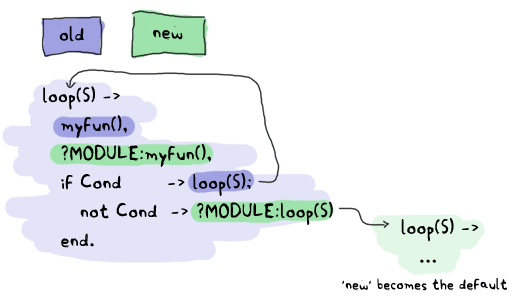
\includegraphics[width=0.7\textwidth]{hot-code-loading.png}
\end{figure}

Учитывая то, что каждому процессу/актору в Erlang для изменения состояния необходимо выполнить рекурсивный вызов, существует возможность загружать совершенно новые версии актора, исполняя внешний рекурсивный вызов.

\colorbox{lgray}
{
\begin{minipage}{1.0\linewidth}
    \textbf{Замечание:} если вы загрузите третью версию модуля в тот момент, когда процесс всё ещё исполняется с использованием первой, этот процесс будет убит виртуальной машиной.
    Она считает, что это был процесс\--сирота, который выполнялся без участия супервизора, или без возможности себя модернизировать (upgrade). 
    Если самая старая версия никем не используется, её просто выбрасывают, а вместо неё остаются более новые.
\end{minipage}
}

Существуют средства, позволяющие связаться с системным модулем, который будет отсылать сообщения при каждой загрузке новой версии модуля.
Вы сможете запускать перезагрузку модуля только при получении такого сообщения, и всегда осуществлять её, используя функцию модернизации кода, скажем \ops{MyModule:Upgrade(CurrentState)}, которая сможет привести структуру данных состояния к требованиям, которые предъявляет новая версия.
Такая обработка с <<подпиской>> автоматически производится фреймворком OTP, который мы скоро начнём изучать.
Для приложения\--напоминалки мы не будем использовать сервер кода, а вместо этого будем посылать из оболочки пользовательское сообщение \ops{code\_change}, после чего будет выполняться очень простая перезагрузка кода.
Вот собственно и все знания, которые нужны для проведения горячей загрузки кода.
Тем не менее, я приведу более общий пример:
\begin{lstlisting}[style=erlang]
-module(hotload).
-export([server/1, upgrade/1]).
 
server(State) ->
    receive
        update ->
            NewState = ?MODULE:upgrade(State),
            ?MODULE:server(NewState);  %% loop in the new version of the module
        SomeMessage ->
            %% do something here
            server(State)  %% stay in the same version no matter what.
    end.
 
upgrade(OldState) ->
    %% transform and return the state here.
\end{lstlisting}

Как видите, наша функция \ops{?MODULE:loop(S)} вписывается в этот шаблон.
\section{Я сказал, прячьте свои сообщения}
\label{i-said-hide-your-messages}
Сокрытие сообщений!
Если хотите, чтобы другие люди могли брать за основу ваш код и процессы, нужно научиться прятать сообщения за функциями интерфейса.
Вот как это сделано в модуле \ops{evserv}:
\begin{lstlisting}[style=erlang]
start() ->
    register(?MODULE, Pid=spawn(?MODULE, init, [])),
    Pid.
 
start_link() ->
    register(?MODULE, Pid=spawn_link(?MODULE, init, [])),
    Pid.
 
terminate() ->
    ?MODULE ! shutdown.
\end{lstlisting}

Я решил зарегистрировать серверный модуль, чтобы в каждый момент времени был запущен только один его экземпляр.
Если бы вам захотелось расширить напоминатель, чтобы его смогли использовать несколько пользователей, было бы неплохо зарегистрировать имена в \href{http://erldocs.com/R15B/stdlib/global.html}{глобальном модуле}, или с помощью \href{http://github.com/uwiger/gproc}{библиотеки gproc}.
Для нужд этого демонстрационного приложения таких средств будет достаточно.

Теперь давайте разберёмся с первым записанным нами сообщением, которое призвано решить проблему подписки.
Исходя из протокола или спецификации, которую я записал выше, напрашивается использование монитора, поэтому мы его здесь и применим.
Если ссылка, полученная в ответ на сообщение о подписке, будет возвращена в сообщении \ops{DOWN}, клиенту станет ясно, что сервер прекратил работу.
\begin{lstlisting}[style=erlang]
subscribe(Pid) ->
    Ref = erlang:monitor(process, whereis(?MODULE)),
    ?MODULE ! {self(), Ref, {subscribe, Pid}},
    receive
        {Ref, ok} ->
            {ok, Ref};
        {'DOWN', Ref, process, _Pid, Reason} ->
            {error, Reason}
    after 5000 ->
        {error, timeout}
    end.
\end{lstlisting}

Далее по списку идёт добавление события:
\begin{lstlisting}[style=erlang]
add_event(Name, Description, TimeOut) ->
    Ref = make_ref(),
    ?MODULE ! {self(), Ref, {add, Name, Description, TimeOut}},
    receive
        {Ref, Msg} -> Msg
    after 5000 ->
        {error, timeout}
    end.
\end{lstlisting}

Обратите внимание, что я решил пересылать клиенту сообщение \ops{\{error, bad\_timeout\}}
Я бы смог также аварийно завершить процесс\--клиент, возбуждая исключение \ops{erlang:error(bad\_timeout)}.
Вопрос о том, как нужно поступать: завершать процесс\--клиент или пересылать сообщение об ошибке, до сих пор обсуждается сообществом разработчиков.
Вот как выглядит альтернативная функция, которая будет возбуждать исключение:
\begin{lstlisting}[style=erlang]
add_event2(Name, Description, TimeOut) ->
    Ref = make_ref(),
    ?MODULE ! {self(), Ref, {add, Name, Description, TimeOut}},
    receive
        {Ref, {error, Reason}} -> erlang:error(Reason);
        {Ref, Msg} -> Msg
    after 5000 ->
        {error, timeout}
    end.
\end{lstlisting}

Далее следует отмена события.
Функцию, выполняющую это действие, мы так и назовём:
\begin{lstlisting}[style=erlang]
cancel(Name) ->
    Ref = make_ref(),
    ?MODULE ! {self(), Ref, {cancel, Name}},
    receive
        {Ref, ok} -> ok
    after 5000 ->
        {error, timeout}
    end.
\end{lstlisting}

Ну и в последнюю очередь, для удобства клиента, мы создадим небольшую функцию, которая будет аккумулировать все сообщения, полученные в течение заданного периода времени.
Если за указанный временной промежуток были получены сообщения, все они передаются вызывающему коду, а функция как можно быстрее завершает работу:
\begin{lstlisting}[style=erlang]
listen(Delay) ->
    receive
        M = {done, _Name, _Description} ->
            [M | listen(0)]
    after Delay*1000 ->
        []
    end.
\end{lstlisting}
\section{Пробный запуск}
\label{a-test-drive}
Теперь вы сможете скомпилировать приложение и совершить его пробный запуск.
Чтобы всё немного упростить, мы напишем специальный Erlang\--овый makefile для сборки проекта.
Откройте в базовой директории проекта файл с названием \ops{Emakefile}.
Файл содержит термы Erlang и задаёт компилятору Erlang рецепт изготовления замечательных свежих и хрустящих \ops{.beam} файлов:
\begin{lstlisting}[style=erlang]
{'src/*', [debug_info,
            {i, "src"},
            {i, "include"},
            {outdir, "ebin"}]}.
\end{lstlisting}

Этот код сообщает компилятору следующее: в файлы необходимо добавить debug\_info (от такой возможности вряд ли стоит отказываться), искать файлы нужно в директориях \ops{src/} и \ops{include/}, а результат компиляции следует поместить в \ops{ebin/}.

\begin{wrapfigure}{r}{0.35\linewidth}
    
\includegraphics[width=1\linewidth]{oven.png}
\end{wrapfigure}

Если открыть командную строку и запустить \ops{erl -make}, все файлы будут скомпилированы, и результат окажется в директории \ops{ebin/}.
Откройте оболочку Erlang командой \ops{erl -pa ebin/}.
Опция \ops{-pa <directory>} сообщает виртуальной машине Erlang, что этот путь необходимо учитывать при поиске модулей.

Можно также запустить оболочку в обычном порядке и исполнить \ops{make:all([load])}.
Этот вызов разыщет файл <<Emakefile>> в текущей директории, проведёт его рекомпиляцию (если файл был изменён) и загрузит новые файлы.

Теперь вы сможете отслеживать тысячи событий (просто замените переменные \emph{DateTime} на любые подходящие значения, которые имеют смысл на текущий момент): 
\begin{lstlisting}[style=erlang]
1> evserv:start().
<0.34.0>
2> evserv:subscribe(self()).
{ok,#Ref<0.0.0.31>}
3> evserv:add_event("Hey there", "test", FutureDateTime).
ok
4> evserv:listen(5).
[]
5> evserv:cancel("Hey there").
ok
6> evserv:add_event("Hey there2", "test", NextMinuteDateTime).
ok
7> evserv:listen(2000).
[{done,"Hey there2","test"}]
\end{lstlisting}

Славно славно славно.
Теперь с помощью созданных нами базовых функций интерфейса, написание клиента должно стать довольно простой задачей.
\section{Добавляем слежение}
\label{adding-supervision}
Для того, чтобы сделать наше приложение более стабильным, мы должны написать ещё один 'перезапускатель'(restarter), наподобие того, что мы написали в \ref{naming-processes} предыдущей главе.
Открывайте файл \href{http://learnyousomeerlang.com/static/erlang/sup.erl}{sup.erl}, именно в нём будет располагаться наш супервизор:
\begin{lstlisting}[style=erlang]
-module(sup).
-export([start/2, start_link/2, init/1, loop/1]).
 
start(Mod,Args) ->
    spawn(?MODULE, init, [{Mod, Args}]).
 
start_link(Mod,Args) ->
    spawn_link(?MODULE, init, [{Mod, Args}]).
 
init({Mod,Args}) ->
    process_flag(trap_exit, true),
    loop({Mod,start_link,Args}).
 
loop({M,F,A}) ->
    Pid = apply(M,F,A),
    receive
        {'EXIT', _From, shutdown} ->
            exit(shutdown); % will kill the child too
        {'EXIT', Pid, Reason} ->
            io:format("Process ~p exited for reason ~p~n",[Pid,Reason]),
            loop({M,F,A})
    end.
\end{lstlisting}

Что\--то похожее мы уже видели в 'перезапускателе', хотя этот код чуть более обобщён и может принимать любой модуль, в котором определена функция \ops{start\_link}.
Процесс, за которым ведётся наблюдение, будет перезапускаться бесконечно, только если сам супервизор не прекратит работу, сгенерировав сигнал выхода.
Вот как можно использовать этот код:
\begin{lstlisting}[style=erlang]
1> c(evserv), c(sup).
{ok,sup}
2> SupPid = sup:start(evserv, []).
<0.43.0>
3> whereis(evserv).
<0.44.0>
4> exit(whereis(evserv), die).
true
Process <0.44.0> exited for reason die
5> exit(whereis(evserv), die).
Process <0.48.0> exited for reason die
true
6> exit(SupPid, shutdown).
true
7> whereis(evserv).
undefined
\end{lstlisting}

Как видите, убийство супервизора также повлечёт смерть его дочернего процесса.

\colorbox{lgray}
{
\begin{minipage}{1.0\linewidth}
    \textbf{Замечание:} мы ознакомимся с более совершенными и гибкими супервизорами в главе о супервизорах OTP.
    Именно их имеют в виду люди, когда говорят о \emph{деревьях контроля (supervision trees)}.
    Здесь мною была показана самая простая форма супервизора, какая только может существовать.
    Она не вполне подходит для использования в рабочем окружении, и не выдерживает сравнения с настоящими супервизорами.

\end{minipage}
}
\section{Пространства имён (или отсутствие таковых)}
\label{namespaces-or-lack-thereof}
\begin{wrapfigure}{l}{0.35\linewidth}
    
\includegraphics[width=1\linewidth]{gentleman.png}
\end{wrapfigure}
Из\--за того, что в Erlang используется плоская структура модулей (нет иерархии), между некоторыми приложеними нередко возникают конфликты.
Примером может послужить широко используемый модуль \ops{user}, который определяется почти в каждом проекте хотя бы один раз.
Это определение пересекается с модулем \ops{user}, который поставляется вместе с Erlang.
Проверку на конфликты можно произвести при помощи функции \href{http://erldocs.com/17.3/kernel/code.html#clash/0}{code:clash/0}.

Для решения проблемы коллизий используют общий шаблон: предваряют каждое имя модуля именем вашего проекта.
В нашем случае модули приложения\--напоминалки должны быть переименованы в \ops{reminder\_evserv}, \ops{reminder\_sup} и \ops{reminder\_event}.

Некоторые программисты идут ещё дальше и добавляют модуль, который назвыается так же как и само приложение.
В этом модуле объединены простые вызовы, которые могут применять программисты во время использования своих програм.
Примером таких вызовов могут послужить функции запуска приложения при помощи супервизора, оформление подписки при работе с сервером, добавление и отмена событий и т.д.

Также важно помнить о существовании других пространств имён, таких как зарегистрированные имена, которые также не должны конфликтовать, имена таблиц баз данных и т.д.

Вот, собственно, и всё, что можно было рассказать о простом параллельном (concurrent) Erlang\--приложении.
Было показано, что мы способны, не особо задумываясь, создавать несколько одновременно исполняющихся процессов: супервизоры, клиенты, серверы, процессы\--таймеры (и мы можем запускать тысячи таких процессов), и т.д.
Их не нужно синхронизировать между собой, нет никаких блокировок, нет явного основного цикла.
Передача сообщений позволила легко разделять наше приложение на несколько модулей с обособленными зонами ответственности и решаемыми задачами.

Вызовы из \href{http://learnyousomeerlang.com/static/erlang/evserv.erl}{evserv.erl} можно использовать для построения клиентов, которые смогут взаимодействовать с сервером событий из\--за пределов виртуальной машины Erlang, и, тем самым сделать программу по\--настоящему полезной.

Но прежде чем мы это сделаем, я рекомендую вам почитать о фреймворке OTP.
Несколько последующих глав будут рассказывать о его составных частях, которые позволят нам писать более надёжные и элегантные приложения.
Большая часть мощи Erlang вытекает из использования этих конструкций.
Это тщательно разработанный и хорошо спроектированный инструмент, который должен знать любой уважающий себя программист на Erlang.
